\chapter{Desenvolvimento}
Este capítulo irá tratar da implementação prática deste trabalho. Para tanto, será dividido em 4 seções: o software de simulação de robótica V-Rep, o sensor \`{a} laser de distância Hokyuo, o modelo de robô utilizado Pioneer P3DX e, por fim, a implementação do algoritmo descrito em 2.X no Matlab.

\section{Software de Simulação Robótica V-Rep}
\paragraph{}
O V-Rep trata-se de um software de simulação robótica desenvolvido pela empresa Coppelia Robotics que, at\'{e} a data de apresentação deste documento, encontra-se em sua terceira versão. Mesmo em sua instalação básica, este software j\'{a} conta com a modelagem de diversos robôs móveis e fixos, bem como uma grande variedade de sensores disponíveis no mercado e utilizados em projetos reais de robótica. N\~{a}o obstante, o software também oferece uma série de modelos para a simulação do ambiente de trabalho do robô, como paredes, esteiras rolantes, dentre outros. Caso o software não ofereça algum modelo específico, este também tem a funcionalidade de poder modelar qualquer outro robôs que não esteja já incluído em sua biblioteca, e também de interfaces para operação dos robôs.

\paragraph{}
Os modelos implementados podem ser programados de 2 formas: através de scripts escritos em linguagem Lua no próprio V-Rep, através da tela de scripts. Ou através da API remota, que como descrito em \cite{copelia1}, tem suporte às seguintes linguagens de programação:
\begin{itemize}
	\item C\textbackslash C++
	\item Python
	\item Java
	\item Matlab
	\item Octave
	\item Urbi
	\item Lua
\end{itemize}

\paragraph{}
Neste trabalho foi utilizado o Matlab para fazer a programação dos modelos, e na seção seguinte será descrito como configurar o V-Rep e o Matlab para para trabalharem em conjunto.

\subsection{Habilitação da API Remota}
\paragraph{}
A habilitação da API remota no lado do servidor, V-Rep, pode ser feita de forma global ou de forma individual, nos scripts do projeto sendo executado. Quando habilitada de forma global, a API pergunte controlar qualquer projeto aberto assim que o V-Rep é executado. Quando a habilitação é feita de forma individual, só é possível controlar o projeto que teve sua simulação iniciada. Sendo assim, com a habilitação individual não é possível utilizar comandos como \texttt{simxStartSimulation}

\paragraph{}
Para habilitar a API de forma individual basta abrir a tela de scripts, acessível através do menu \emph{Tools$\rightarrow$Scripts}, e adicionar no topo do script em que se deseja habilitar a API a seguinte linha, onde \emph{<porta>} corresponde à porta da conexão:

\begin{flushleft}
	\texttt{simExtRemoteApiStart(\emph{<porta>})}
\end{flushleft}

\paragraph{}
Para habilitar a API de forma global primeiramente é necessário criar um arquivo chamado \emph{remoteApiConnections.txt}, dentro da pasta raiz do V-Rep. Dentro deste arquivo devem estar contidas as seguintes linhas:

\begin{flushleft}
	\texttt{portIndex@\_port = \emph{<porta>}} \newline
	\texttt{portIndex@\_debug = \emph{true/false}} \newline
	\texttt{portIndex@\_syncSimTrigger = \emph{true/false}}
\end{flushleft}

Neste caso @ corresponde ao índice, que servirá para identificar os parâmetros introduzidos. O primeiro comando especifica a porta para aquele índice, o segundo habilita ou desabilita debug através da porta, e o último habilita ou desabilita execução síncrona do V-Rep com o programa externo através da porta especificada pelo índice.

\paragraph{}
Após a habilitação da API no lado do servidor, é necessário também habilitá-la junto ao programa que será utilizado para controlar os modelos do V-Rep. No caso deste trabalho, será explicado como configurar a API no Matlab. Primeiramente é necessário adicionar os seguintes arquivos na mesma pasta do projeto do Matlab:

\begin{itemize}
	\item \emph{remApi.m}
	\item \emph{remoteApiProto.m}
	\item \emph{remoteApi.dll}
\end{itemize}

Os arquivos \emph{.m} podem ser achados na pasta \sloppy{\emph{<raiz\_V-Rep>$\backslash$V-REP\_PRO\_EDU$\backslash$programming$\backslash$remoteApiBindings$\backslash$matlab$\backslash$matlab}}. O arquivo \emph{.dll} pode ser encontrado na pasta \sloppy{\emph{<raiz\_V-Rep>$\backslash$V-REP\_PRO\_EDU$\backslash$programming$\backslash$remoteApiBindings$\backslash$lib$\backslash$lib$\backslash$(64Bit ou 32Bit)}}. É importante ressaltar que as bibliotecas com a extensão \emph{.dll} são usada no sistema Windows, para o caso do Linux e do Mac OsX as extensões dos arquivos serão diferentes, porém estarão contidas na mesma pasta.

\paragraph{}
Após estes passos, o ambiente de trabalho já está configurado e é possível iniciar uma conexão com o V-Rep. Para tanto primeiramente é necessário criar um objeto de controle do V-Rep utilizando-se a função \emph{remApi.m} importada previamente, e especificando a biblioteca também importada previamente. Após isto deve-se utilizar o objeto para iniciar a conexão com o V-Rep utilizando-se o comando \texttt{simxStart}, que retornará o id da conexão estabelecida ou -1 caso a tentativa de conexão tenha fracassado:

\begin{flushleft}
	\texttt{vrep = remApi(\lq{remoteApi}\rq)} \newline
	\texttt{id = vrep.simxStart(\lq{127.0.0.1}\rq, 19997, true, true, 2000, 5);}
\end{flushleft}

\subsection{Conexão dos Elementos no V-Rep}

\paragraph{}
Após a configuração do ambiente de trabalho, é necessário inserir modelos necessários ao projeto para que a simulação possa ser executada. O V-Rep possui um sistema de hierarquia do tipo \emph{pai-filho}, sendo assim o objeto pai consegue obter e alterar propriedades do objeto filho, mas o objeto filho não consegue fazer o mesmo com o pai. No caso deste projeto foi utilizado o sensor de distância à laser Hokuyuo URG-04LX-UG01 acoplado ao robô Pioneer P3DX, para isso é necessário que o sensor seja filho do objeto pai robô. Caso esta hierarquia não seja obedecida, quando a simulação for iniciada, o robô se moverá mas o sensor não, mesmo que este tenha sido corretamente posicionado no local desejado. Para tornar um objeto filho de outro, é necessário posicioná-lo dentro da árvore hierárquica do objeto pai, como mostrado na figura \ref{fig:arvore-v-rep}.
	
\begin{figure}[h]
	\centering
	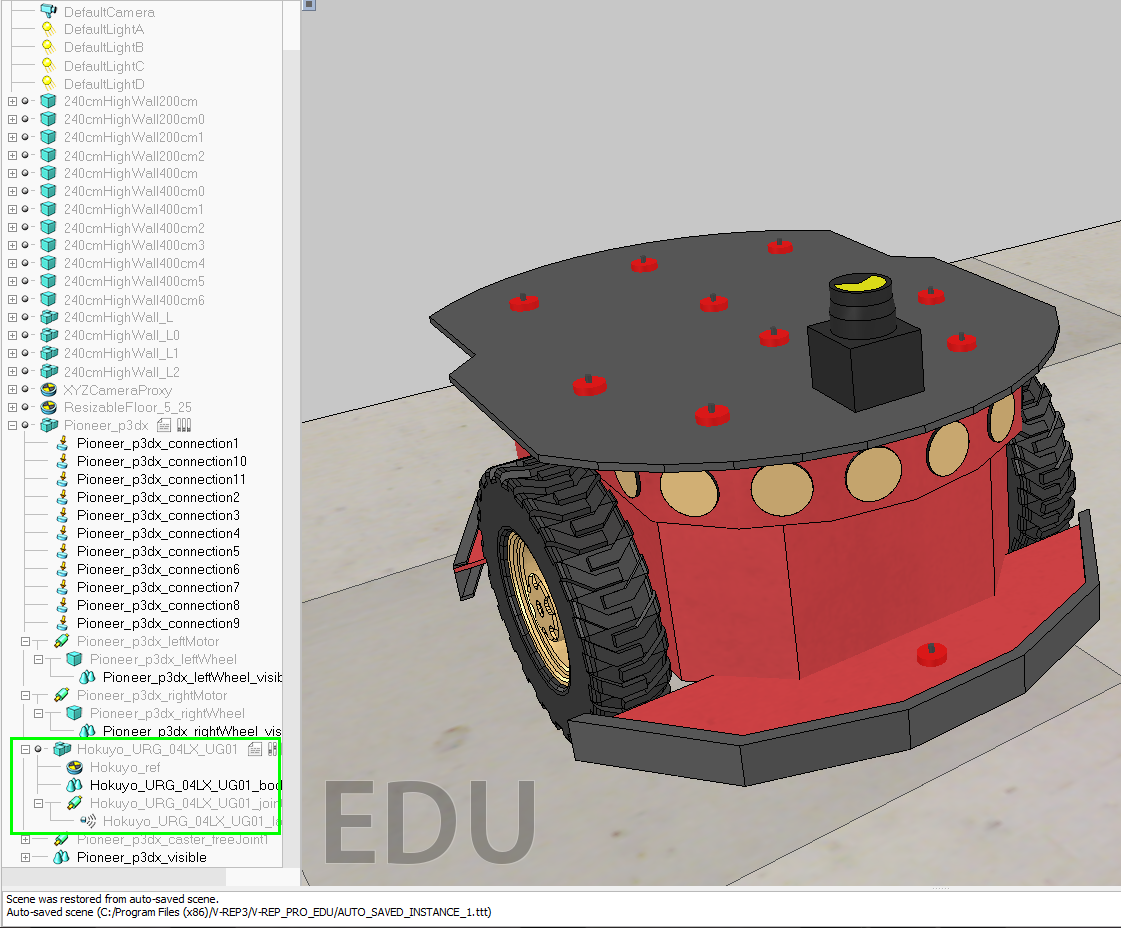
\includegraphics[width=0.7\textwidth]{imagens/insercao_elementos_vrep}
	\caption{Árvore Hierárquica V-Rep}
	\label{fig:arvore-v-rep}
\end{figure}

\paragraph{}
Na figura \ref{fig:arvore-v-rep} também é possível observar a posicionamento do sensor, que terá seu \emph{frame} movimentado na mesma direção, sentido e velocidade da movimentação do \emph{frame} do robô, o objeto pai.



